\section{Bevægelsessensor}\label{sec_design_LSM9DS1}
\textit{I dette afsnit designes, implementeres og testes accelerometeret og gyroskopet, som benyttes til opsamling af data under aktiviteter.}

\subsection{Design} \label{design_lsm}
Der benyttes et IC af typen LSM9DS1, der kræver 2,4-3,6~V for at være funktionel. Denne indeholder magnometer, gyroskop og accelerometer, hvoraf magnometeret ikke bliver benyttet.\fxnote{Magnometeret benyttes til måling af givne paramtere på et magnetfelt}~\citep{Jimb02016,STMicroelectronics2016} \\ 
Arbejdsområderne for accelerometeret og gyroskopet er valgbare, hvoraf det er muligt at indstille accelerometeret til $\pm$1, $\pm$4, $\pm$8 eller $\pm$16~g, og gyroskopet kan indstilles til $\pm$245, $\pm$500 eller $\pm$2000~dps.~\citep{Jimb02016,STMicroelectronics2016} På baggrund af kravene opstillet i \secref{Sec:krav}, vælges accelerometerets arbejdsområde til $\pm$16~g og gyroskopets arbejdsområde til $\pm$2000~dps.\fxnote{værdien på 500 er få tæt på værdien i pilotforsøget, og da vi ikke ved, hvad der sker under accleration, så vælges 2000~dps.} 

LSM9DS1 har seks frihedsgrader når magnometeret fravælges, hvilket betyder at den måler i x-, y- og z-aksen for henholdsvis accelerometeret og gyroskopet, som kan ses på \figref{vores_IC}.~\citep{STMicroelectronics2016}\newline 
\begin{figure}[H]
	\centering
	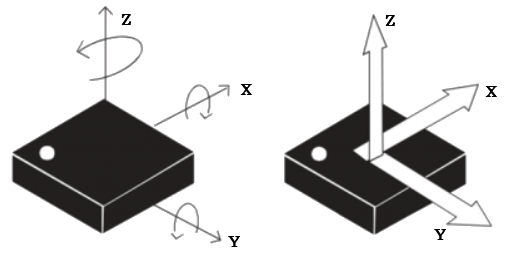
\includegraphics[scale=0.4]{figures/cDesign/LSM9DS1.png}
	\caption{På figuren ses akserne på LSM9DS1 for gyroskopet, der ses til venstre, og accelerometeret, der ses til højre.~\citep{Jimb02016}~(Modificeret)}
	\label{vores_IC}
\end{figure}\vspace{-0.25cm}
Sensorens opbygning fremgår af \figref{fig:IC_pins}, hvor der er fire pins på venstre side og ni pins på højre side af sensoren. ICens pins på højre side vil ikke blive benyttet.\\
De fire pins på venstre side af ICen bliver benyttet til spændingstilkobling samt til at læse sensorens outputdata. GND og VDD er pins til henholdsvis jord og spændingsforsyning, mens SDA er I$^2$C datapin, hvor data bliver sendt og modtaget. SCL er en seriel clock, der blandt andet sørger for synkron dataopsamling.
\begin{figure}[H]
	\centering
	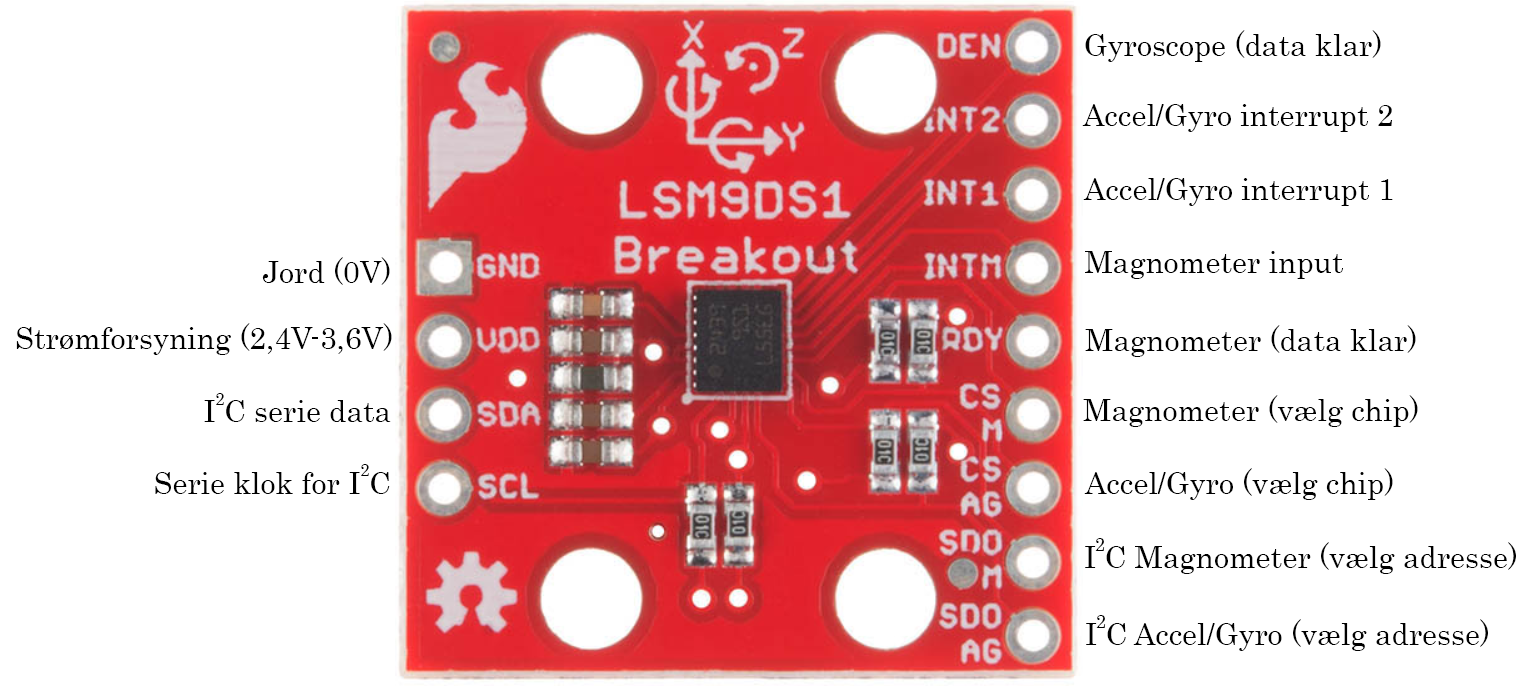
\includegraphics[scale=0.3]{figures/cDesign/accelerometeret.png}
	\caption{Figuren viser pinkonfigurationen af LSM9DS1.~\citep{Jimb02016}~(Modificeret)}
	\label{fig:IC_pins}
\end{figure}\vspace{-0.25cm}
LSM9DS1 er en digital sensor, hvormed de analoge signaler konverteres til digitale i ICen ved hjælp af en indbygget 16~bits ADC. Derfor skal sensoren konfigureres til en given samplingsfrekvens for ADCen. Ifølge \secref{krav_adc} skal accelerometret sample med mindst 450~Hz. Det fremgår af databladet for ICen, at accelerometret kan konfigureres til seks forskellige samplingsfrekvenser. En samplingsfrekvens på 476~Hz har mindst afvigelse til den ønskede samplingsfrekvens, hvorfor denne vælges. \\
Gyroskopet skal samples med mindst 60~Hz, men ifølge gyroskopets datablad kan den indstilles til 59,5~Hz eller 119~Hz, hvorfor samplingsfrekvensen vælges til 119~Hz.

Det AD-konverterede outputsignal fra ICen kan benyttes med en SPI og en I$^{2}$C kommunikationsprotokol. Den benyttede mikrokontroller, CY8CKIT-043 PSoC 4-M, besidder begge kommunikationsprotokoller. I$^{2}$C kommunikationsprotokollen bliver benyttet, idet der skal være modtagelse og afsendelse af data mellem ICen og MCUen. For at kunne opsætte I$^{2}$C bussen for PSoC~4200M er det påkrævet, at der benyttes to pull-up modstande. Ved at benytte to modstande med en værdi på 4,7~$k\Omega$ bliver I$^{2}$C bussen konfigureret til at operere i standard tilstand som er en hastighed på 0-100~kB per sekund.~\citep{CYPRESS2016} \\
For at kunne benytte I$^{2}$C bussen er det yderligere påkrævet at kode ICen, således der skrives og læses fra et givent dataregister i ICen. På \figref{Fig:master_slave} ses kommunikationen mellem en master og en slave, hvoraf slaven i dette tilfælde er ICen og masteren er GAP peripheral.\fxnote{Og dette kan ikke vendes om, ICen vil ALTID være slaven} 
\begin{figure}[H]
	\centering
	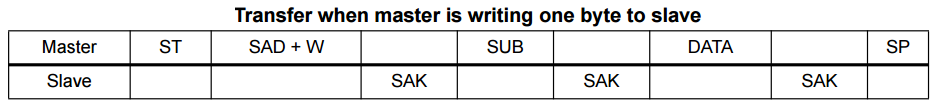
\includegraphics[scale=0.75]{figures/cDesign/Sensor_write_read2.png}
	\caption{På figuren ses metoden for overførsel af én byte mellem slave og master ved brug af I$^{2}$C kommunikationsprotokol.~\citep{STMicroelectronics2016}~(Modificeret)}
	\label{Fig:master_slave}
\end{figure}\vspace{-0.25cm}
Det fremgår af \figref{Fig:master_slave}, at MCUen skriver en startkode (ST) til ICen for at påbegynde kommunikationen mellem master og slave. Herefter skriver masteren en adresse til slaven (SAD + W) for at starte kommunikationen. Slaven godkender (SAK) oprettelsen af kommunikationen, hvorefter masteren sender en adresse (SUB) til slaven, som bestemmer hvorfra sensoren skal sende data. Når slaven har godkendt (SAK) dette, hentes data over på masteren (DATA). Slaven fortæller, at én byte er sendt (SAK). Afslutningsvist skriver masteren en stop kode til slaven (SP), hvorefter kommunikationen afbrydes.

Gyroskopet i LSM9DS1 forbruger 4~mA og accelerometeret forbruger 0,6~mA, når begge sensorer benyttes under normale forhold~\citep{Jimb02016}\fxnote{hvor Vdd er forsynet med 2,2~V og temperaturen er 25 grader}. For at sikre en høj batterilevetid, er det væsentligt at gyroskopet er aktiveret så kort tid som muligt. Det fremgår af databladet for ICen, at det er muligt at slukke begge sensorer, at benytte accelerometeret alene eller benytte accelerometeret og gyroskopet sammen. Der kan yderligere spares strøm ved brug af gyroskopet, hvis der vælges en lavere samplerate. Disse apspekter vil blive omtalt i \secref{sec:diskussion} samt \secref{sec:perspektivering}\\ % alt efter hvor 
 
\subsection{Implementering}
MCUen kræver to eksterne pull-up modstande tilkoblet for at opsætte I$^{2}$C bussen, hvilket fremgår af \secref{design_lsm}. To eksterne modstande på 4,7~$k\Omega$ forbinder henholdsvis SCL og VDD samt SDA og VDD, hvilket gør I$^{2}$C bussen tilgængelig for dataoverførsel.

I PSoC Creator indhentes det analoge komponent I2CM. Denne skaber en I$^2$C forbindelse imellem MCUen og ICen samtidig med, at den indstiller MCUen til at være master. Topdesignet for I2CM modulet konfigureres ydermere til at have sensorens SDA og SCL pins koblet til MCUen på de valgte pins, som er henholdsvis pin 1.1 og pin 1.0. Disse fremgår i \appref{MCU_stor}.\\
MCUen skal kunne modtage data fra sensoren, hvilket gøres ved at implementere en algoritme i MCUen. Algoritmen skriver til den hex-adresse, som er registeradressens dataoutput for accelerometeret og gyroskopet. Således kan MCUen som master skrive til accelerometret eller gyroskopet. Det fremgår af databladet, at hexkoden '79' konfigurerer gyroskopet til de ønskede indstillinger på 2000~dps og en samplingsfrekvens på 119~Hz.~\citep{STMicroelectronics2016} \\
Der ønskes at benytte en samplingsfrekvens på 476~Hz og et arbejdsområde på $\pm$16~g for accelerometeret. Det fremgår af registeret, at der skal skrives til hex-adressen 'A8' for at konfigurere accelerometeret til disse indstillinger. Der benyttes ikke interrupt benet på ICen, hvorved MCUen henter data med højere frekvens, end ICen er indstillet til at sample med. MCUen henter som resultat af dette data ind hele tiden, som er hurtigere end ICens samplingsfrekvens. Der skal derfor oprettes et delay på MCUen som sørger for, at der kun hentes data fra ICen med en frekvens på 476~Hz. Ved en frekvens på 476~Hz, er der 0,002101~sekunder mellem hver sample. For at kunne bestemme det delay som sikrer, at der samples med 476~Hz for MCUens vedkommende, da undersøges antallet af bytes modtaget uden delay. Realterm benyttes til at måle det antal karakterer, som modtages over en periode på 30~sekunder. Det fremgår heraf, at Realterm modtager 56.035 karakterer på 30~sekunder. Det kan derfor bestemmes, hvilken varighed der er mellem disse samples, hvilket fremgår af \eqref{fucking_delay}.
\begin{equation}\label{fucking_delay}
\frac{1~sekund}{\left(\frac{56.035~karakterer}{30~sekunder}\right)} = \text{0,000535~sekunder}
\end{equation} 
Det ses, at der er 0,000535~sekunder mellem hver sample for MCUen. Derfor er forskellen, mellem ICens og MCUens, varigheder mellem samples på:
\begin{equation}\label{eq:delay_halloej}
0,002101~sekunder~-~0,000535~sekunder~=~0,001565~sekunder
\end{equation} 
Det fremgår af \eqref{eq:delay_halloej}, at forskellen mellem de to varigheder er på 0,001565~sekunder. Ved at indsætte et delay på 0,001565~sekunder bliver frekvensen for MCUen:
\begin{equation}\label{qe:hader_delay}
\frac{1}{0,000535~+~0,001565}~=~476,19~Hz
\end{equation}
I \eqref{qe:hader_delay} adderes eksekveringstiden per sample sammen med det beregnede delay, således en korrekt frekvens for MCUen kan opsættes. 

\subsection{Test}
Testen udføres på baggrund af de opstillede krav og tilhørende afvigelser opstillet i henholdsvis \secref{krav:acc} og \secref{krav:gyro}. Kravene til accelerometeret og gyroskopet er som følger:\\
Accelerometeret skal:
\begin{itemize}
\item Have et arbejdsområde på $\pm$16 g. Der accepteres ikke et mindre arbejdsområde.
\item Angive korrekt g-påvirkning under kontrollerede forhold. Der accepteres en afvigelse på 5\%.
\item ICens ADC skal have en samplingsfrekvens på mindst 450~Hz. Der accepteres ikke en samplingsfrekvens under 450~Hz.
\end{itemize}
Gyroskopet skal:
\begin{itemize}
\item Have et arbejdsområde på mindst 334,69~dps. Der accepteres ikke et arbejdsområde herunder.
\item Samples med mindst 60~Hz af ICens ADC. Der accepteres ikke en samplingsfrekvens under 60~Hz.
\end{itemize}
Eftersom ADCen, der benyttes til at konvertere det analoge signal fra accelerometret og gyroskopet, er en indbygget komponent i ICen, vanskeliggøres en test heraf. Det antages derfor, at ADCens sampling og sensitivitet er tilsvarende de konfigurerede indstillinger, som fabrikanten foreskriver i databladet.~\citep{STMicroelectronics2016}

Accelerometeret er indstillet til $\pm$16~g, hvorfor det antages, at den kan registrere bevægelser op til $\pm$16~g. Ifølge accelerometerets andet krav skal det angive korrekt g-påvirkning med en maksimal afvigelse på 5\%. Dette testes ved at påvirke sensorens y-akse med $\pm$1~g. Det har ikke været muligt at teste accelerometerets maksimale arbejdsområde. En måde hvorpå dette kan testes, er ved brug af en maskine som kan indstilles til at påføre accelerometeret en g-påvirkning alt efter dets sensitivitet. 

ICens accelerometer har en sensitivitet på 0,000732~g per LSB~\citep{STMicroelectronics2016}. Outputtet fra sensoren er low byte og high byte, hvilket bliver bitskiftet og derefter adderet i MCUen, hvormed output fra MCUen er i LSB. For at omregne dette output til g skal outputtet multipliceres med sensitiviteten, hvilket sker i tredje kolonne i \tabref{tab:test_sensor} \\
Accelerometerets y-akse testes ved at måle dets output, når denne akse bliver påvirket i horisontal retning placeret på et bord. Ved denne placering bør sensoren y-akse have et output svarende til 0~g. Efterfølgende placeres sensoren med y-aksen i vertikal retning, hvor aksen teoretisk burde påvirkes med $\pm$1~g. Inden målingen testes fladen, der måles på med vaterpas for at sikre, at kun den ønskede akse påvirkedes i vertikal retning. I \tabref{tab:test_sensor} ses resultatet af testen. 
\begin{table}[H]
\centering
\begin{tabular}{cccc}
	\hline
	\cellcolor[HTML]{C0C0C0}\begin{tabular}[c]{@{}c@{}}Teoretisk påvirkning \\ {[}g{]}\end{tabular} & \cellcolor[HTML]{C0C0C0}\begin{tabular}[c]{@{}c@{}}Output fra MCU \\ {[}LSB{]}\end{tabular} & \cellcolor[HTML]{C0C0C0}\begin{tabular}[c]{@{}c@{}}Output fra MCU \\ {[}g{]}\end{tabular} & \cellcolor[HTML]{C0C0C0}\begin{tabular}[c]{@{}c@{}}Afvigelse \\ {[}\%{]}\end{tabular} \\ \hline
	0 & 19 & 0,014 & 1,4 \\ \hline
	+1 & 1368 & 1,003 & 0,3 \\ \hline
	-1 & -1356 & -0,993 & -0,7 \\ \hline
\end{tabular}
	\caption{I tabellen ses resultatet fra testen af accelerometerets y-akse. For at omregne MCUens output fra LSB til g-påvirkning multipliceres outputtet med accelerometerets sensitivitet.}
	\label{tab:test_sensor}
\end{table}\vspace{-0.25cm}
Det ses i \tabref{tab:test_sensor}, at sensorens accelerometer har en afvigelse på -0,7\% til 1,4\%, hvilket overholder den accepterede afvigelse på 5\%. Det er ydermere antaget, at accelerometeret overholder arbejdsområdet på den indstillede værdi $\pm$16~g.

Gyroskopet i ICen har en sensitivitet på 0,070~dps per LSB, når den måler med 2000~dps. Ifølge krav til gyroskopet i \secref{krav:gyro} skal sensoren have et arbejdsområde på mindst 334,69~dps, hvilket overholdes ved valg af 2000~dps. Outputtet fra gyroskopet gives ligeledes i LSB, hvorfor eksempelvis 360~dps, der svarer til én rotation i sekundet, giver et output på 5.142. Det er imidlertid ikke muligt for projektgruppen at teste, hvorvidt gyroskopet giver korrekt output. Dette kræver en kontrolleret cirkulær acceleration om en given akse, hvilket påkræver udstyr, som ikke er tilgængeligt. Hvis sådant udstyr havde været tilgængelig, ville det være fordelagtigt med en cirkulær plade, hvis omdrejninger er kontrollerbare. Derved kan den indstilles til for eksempel én omdrejning i sekundet, og i så fald bør gyroskopet måle 360~dps og give et output på 5.152.
%
%
%Accelerometrets sensitivitet ved 16 g målinger: 0,732 mg/LSB
%Hvor LSB er 2*16/2^16 = 0.0078125
%(Man får et output på ca. 1350 fra acc, hvilket giver næsten 1 ganget med 0,732 mg/LSB)
%
%Gyroskopets sensitivitet med 2000~dps målinger: 70 mdps/LSB (17,5 hvis 500)
%Hvor LSB er 2*2000/2^16 = 0.97656
%()